\chapter{Data}
\label{chap:data}
% introduction to Herschel
\section{\textit{Herschel} column-density maps}
\subsection{Introduction}
The main source of data in this work stems from ESA's \textit{Herschel} Space Observatory \cite{pilbratt2010herschel}, which was launched in 2009 with the goal of observing in the far-infrared and submillimetre wavelengths. 
\textit{Herschel} was equipped with three main instruments: the Photodetector Array Camera and Spectrometer (PACS), the Spectral and Photometric Imaging Receiver (SPIRE), and the Heterodyne Instrument for the Far Infrared (HIFI). These instruments allowed \textit{Herschel} to observe a wide range of astronomical phenomena, including star formation and galaxy evolution.
\textit{Herschel}'s mission lasted until 2013, enabling unprecedented studies of the cold and dusty regions of space.

%introduction to Orion's data
\textit{Herschel}'s observations of Orion, the target of this work, were part of the \textit{Herschel} Gould Belt Survey (HGBS). This survey aimed to map the nearby star-forming regions in the Gould Belt, a flat structure of a few hundred parsecs inclined by approximately 20$^{\circ}$ with respect to the galactic plane \cite{andre2010herschel}.
The clouds covered by the HGBS span a wide range of physical and environmental conditions, from very active, cluster-forming complexes such as the Orion A and B giant molecular clouds (GMCs) to quiescent regions with no star formation activity at all.

% grain properties
\subsection{Dust emission maps}
In the interstellar medium, dust typically has temperatures T$_{\mathrm{dust}}$ around $20$ K and emits thermal radiation that can be approximated by a modified blackbody, peaking at far-infrared (FIR) and submillimetre (mm) wavelengths. 
This thermal dust emission represents the dominant source of FIR and mm-continuum radiation in galaxies, as it can be recognized in Figure \ref{fig:dust_emission_blackbody}. 

\begin{figure}
    \centering
    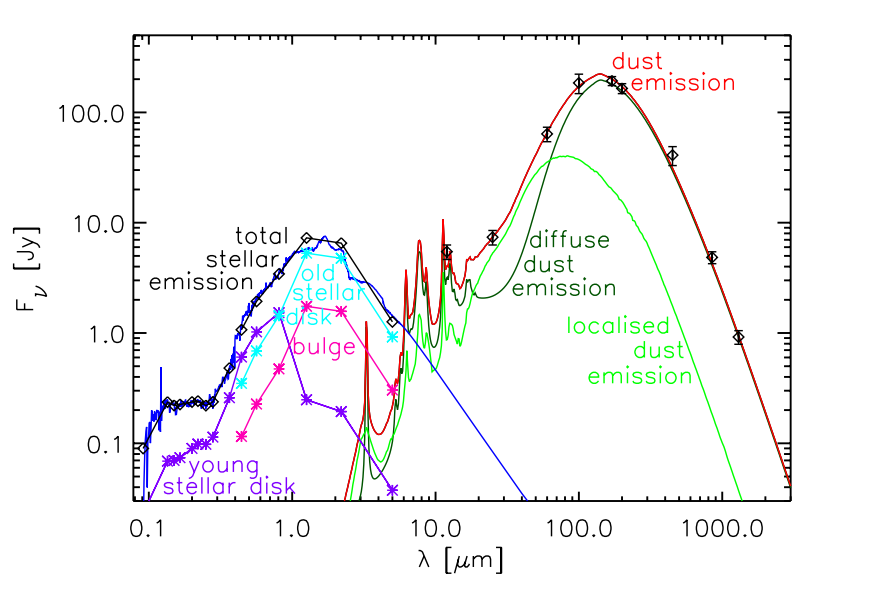
\includegraphics[width=0.75\textwidth]{figures/dust_emission_blackbody.png}
    \caption{LALALA \cite{popescu2011modelling}}
    \label{fig:dust_emission_blackbody}
\end{figure}

Dust grains absorb ultraviolet (UV) and near-infrared (NIR) photons from stars, reprocessing this stellar radiation and re-emitting it at longer wavelengths. 
Because dust is highly efficient at radiating energy, it reaches and maintains relatively low equilibrium temperatures \cite{hildebrand1983determination}. 
Observations of dust emission hence provide a powerful tool to estimate the column density of dust and gas along the line of sight.

% a picture, bit of history
Using mm continuum dust emission to measure column density offers several advantages over traditional extinction-based methods: it can probe much higher column densities where extinction becomes saturated or unreliable, it often provides better angular resolution, and it remains effective even in regions heavily obscured by dust where extinction mapping fails \cite{draine2003interstellar}. Moreover, continuum observations allow simultaneous determination of both dust temperature (T$_{\mathrm{dust}}$) and gas column density (N(H$_2$)), which is essential for characterizing dense molecular clouds. In extragalactic studies, where individual stars cannot be resolved, dust emission often represents the only viable method for estimating gas masses.

However, these methods also involve significant assumptions and uncertainties. Different approaches to estimate column density are conceptually equivalent but may yield different results due to methodological degeneracies. One key source of uncertainty arises from the poorly constrained dust opacity, $\kappa$, which depends on the composition, size distribution, and physical properties of dust grains. Variations in $\kappa$ directly affect the derived column densities, introducing systematic uncertainties into the analysis.

The data used in this work are \textit{Herschel} column-density maps of the Orion A and B giant molecular clouds. These maps were created by combining data from PACS and SPIRE instruments, which observed at different wavelengths to capture the dust emission across the clouds.

% Technicalities of the instruments (what do they measure and how, advantages and disadvantages, etc.)
Specifically, PACS provided imaging photometry in the 60-210 $\mu m$ wavelength range, using two filled silicon bolometer arrays with 16 $\times$ 32 and 32 $\times$ 64 pixels. In photometric mode, PACS simultaneously imaged two bands: either 60-85 $\mu m$ or 85-125 $\mu m$, along with 125-210 $\mu m$, covering a field of view of approximately 1.75 $\times$ 3.5 arcminutes with near-Nyquist sampling \cite{poglitsch2010photodetector}. These bands are particularly sensitive to warmer dust components.

SPIRE extended the coverage to longer wavelengths, better tracing colder dust. Its photometer operated in three broad bands centered at 250 $\mu m$, 350 $\mu m$, and 500 $\mu m$, well-suited for mapping large-scale dust emission from the cold interstellar medium \cite{griffin2010herschel}. 

The combination of PACS and SPIRE photometric data allows for the characterization of the dust spectral energy distribution (SED) across a broad range of temperatures. The relative throughputs of the two instruments can be seen in Figure \ref{fig:pacs_spire_throughputs}, on top of black body radiation for typical temperatures of dust. This broad wavelength coverage enables accurate fitting of modified blackbody models to derive dust temperatures, column densities, and emissivity properties.

% Mabye more on the above once you describe better the process below
\begin{figure}
    \centering
    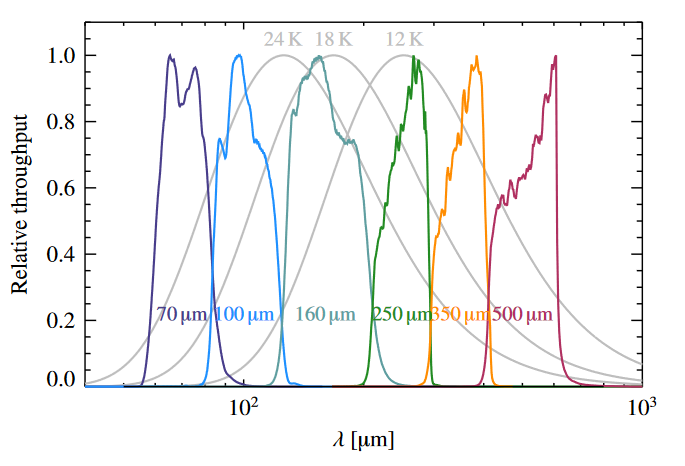
\includegraphics[width=0.75\textwidth]{figures/relative_throughputs_PACS_SPIRE.png}
    \caption{LALALA \cite{lombardi2014herschel}}
    \label{fig:pacs_spire_throughputs}
\end{figure}

\subsection{Derivation of column density maps}

The data (what kind of data) was downloaded from archive (lombardi et al 2014). Properties and such

How do you go from what PACS and SPIRE measure to dust emission maps?

% Going from dust opacity maps to column density maps... 

% Multi-freq. fit allows to solve
%  \& simul

%  Fully characterised by Herschel
% in one go

% tau maps of Orion A and B

Technicalities of the data (good and bad stuff) -> Lombardi et al.

Specific to these maps (coverage and such)

\subsection{Data pre-processing}
Maybe before?
The data were pre-processed using the Herschel interactive processing environment (HIPE, Ott 2010) version 10.0.2843, and the latest version of the calibration files.

\section{YSOs}
Extra: YSOs data? TBD

